\documentclass[twoside]{article}%{combine}
%\usepackage{url}
\usepackage{../../tex/html}
\usepackage{epstopdf}
\usepackage{amsfonts,amsmath,color,amsthm,amssymb, enumerate, bbm, subfig}
\usepackage{graphicx}
%\usepackage[DIV=14,BCOR=2mm,headinclude=true,footinclude=false]{typearea}
%\usepackage[font=small,labelfont=bf]{caption}
\usepackage{hyperref}
\usepackage{tikz, etoolbox}

\usetikzlibrary{shapes}
\usetikzlibrary{arrows}
%\usepackage[margin=1in]{geometry}
\usepackage{graphicx,amsmath,gentium,tikz,caption}
\usetikzlibrary{patterns}
\usetikzlibrary{matrix,arrows,positioning,shapes}
\usetikzlibrary{arrows.meta}
\tikzset{
  a/.style={-{Stealth[scale=1.3,angle'=45]},semithick}
}
%\usepackage{xfrac,fontspec,unicode-math}
%\setmathfont[version=cambria]{Cambria Math}
%\mathversion{cambria}
\usepackage[letterpaper, portrait, margin=1.1in]{geometry}
\usepackage{amsmath,amsthm}
\usepackage{mathtools}
\newtheorem*{definition}{Definition}
\usepackage{tcolorbox}
\tcbset{colback=white,colframe=black}
\everymath{\displaystyle}

\makeatletter
\@ifundefined{namelength}{
\newlength{\namelength}
\settowidth{\namelength}{{\bf \Large Name: }}
\newlength{\namelinelength}
\setlength{\namelinelength}{\textwidth}
\addtolength{\namelinelength}{-\namelength}
}{}

\@ifundefined{vs}{
\newcommand*{\vs}[1]{\par
  \vspace*{#1\baselineskip}%
  \@afterindentfalse
  \@afterheading
}
}{}
\makeatother



\def\fancytitle#1#2#3{
      \centerline{\framebox{\framebox{ \parbox{.8\textwidth}{ \bf ENGRI 1101 \hfill
      Engineering Applications of OR \ \ \ \  Fall 2020 \hfill #3 #1 \\
\mbox{ }\hfill
      \hfill\mbox{ } \\[1mm] \mbox{ } \hfill{\Large \bf #2}\hfill
      \mbox{ }} }}}
      
\vs 2
}

\def\handout#1#2{\fancytitle{#1}{#2}{Handout}}
\def\review#1#2{\fancytitle{#1}{#2}{Review}}
\def\homework#1#2{\fancytitle{#1}{#2}{Homework}}
\def\exercises#1{\fancytitle{}{#1}{Exercises}}
\def\solution#1#2{\fancytitle{#1}{#2}{Solutions}}
\def\final#1#2{\fancytitle{#1}{#2}{Final}
      \noindent {\bf \Large Name:} \rule{\namelinelength}{0.5pt}
      \vspace*{\baselineskip}}
\def\prelim#1#2{\fancytitle{#1}{#2}{Prelim}
      \noindent {\bf \Large Name:} \rule{\namelinelength}{0.5pt}
      \vspace*{\baselineskip}}
\def\quiz#1#2{\fancytitle{#1}{#2}{Quiz}
      \noindent {\bf \Large Name:} \rule{\namelinelength}{0.5pt}
      \vspace*{\baselineskip}}
\def\lab#1#2{\fancytitle{#1}{#2}{Lab}
      \noindent {\bf \Large Name:} \rule{\namelinelength}{0.5pt}
      \vspace*{\baselineskip}}
\def\prelab#1#2{\fancytitle{#1}{#2}{Prelab}
      \noindent {\bf \Large Name:} \rule{\namelinelength}{0.5pt}
      \vspace*{\baselineskip}}

\raggedbottom

\begin{document}

\prelab {4}{The Maximum Flow Problem}

\noindent
\textbf{Objectives:}

\begin{itemize}
\item Introduce the maximum flow problem.
\item Demonstrate how to solve the maximum flow problem by the
  Ford-Fulkerson algorithm.
\end{itemize}

\noindent
\textbf{Key Ideas:}

\begin{minipage}[t]{.45\linewidth}
  \begin{itemize}
  \item sink and source nodes
  \item flow
  \item feasible flow
  \item value of flow
  \item cuts
  \end{itemize}  
\end{minipage}
\hfill
\begin{minipage}[t]{.45\linewidth}
  \begin{itemize}
  \item capacity of cut
  \item max-flow min-cut theorem
  \item integrality properties
  \item sensitivity analysis
  \end{itemize}
\end{minipage}

\vspace{1em}

\noindent
\textbf{Reading Assignment:}
\begin{itemize}
\item
Read Handout 5 on the maximum flow problem.
\end{itemize}

\noindent
\textbf{Prelab Exercise:}


\noindent
For the following graph, compute the maximum flow from node 1 to node
3 in any way you like. (The numbers on the arcs are capacities.) Can you give a convincing argument that you
have found an optimal solution?
%% REMOVED Fall 2013 because I didn't cover cuts until the day of the lab
% Can you find a cut of minimum capacity? What is the capacity of the minimum cut? What is the value of the maximum flow?

\bigskip

\begin{center}
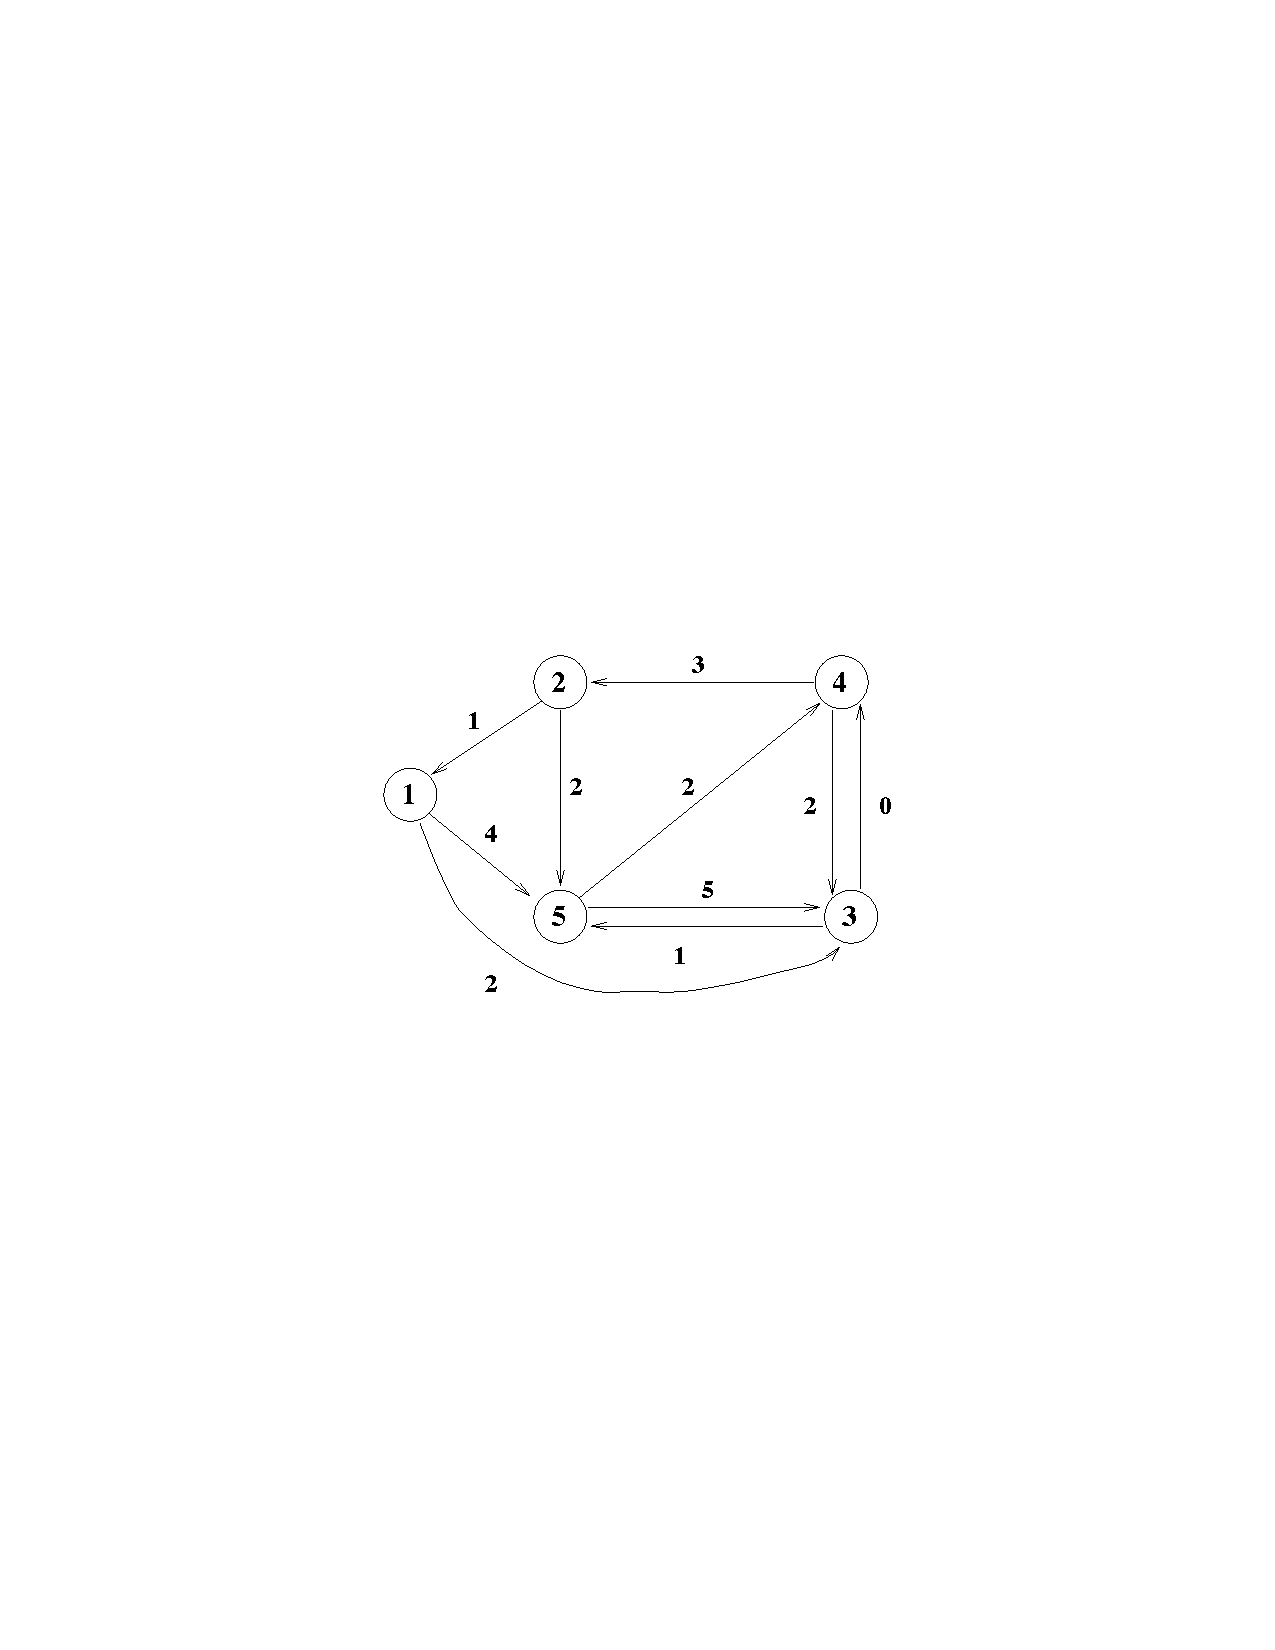
\includegraphics[height= 2in]{prelab4_fig1.pdf}
\end{center}

\end{document}
